\begin{figure}[ht]
	\begin{subfigure}[b]{0.32\linewidth}
		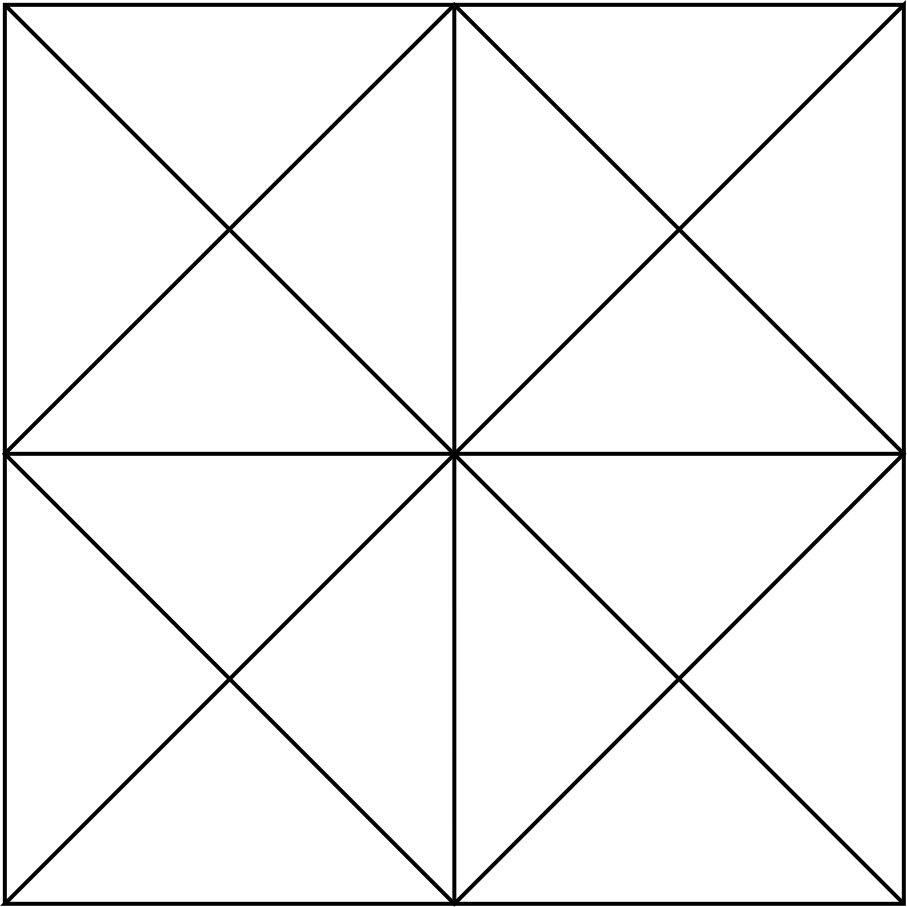
\includegraphics[width=\linewidth]
		{data/synthetic_meshes/square_tesselation_4tri_Dirac_delta_1_v13_f16_wireframe.png}
		\caption{R=1, wireframe}\label{fig:sq2.a}
	\end{subfigure}
	\begin{subfigure}[b]{0.32\linewidth}
		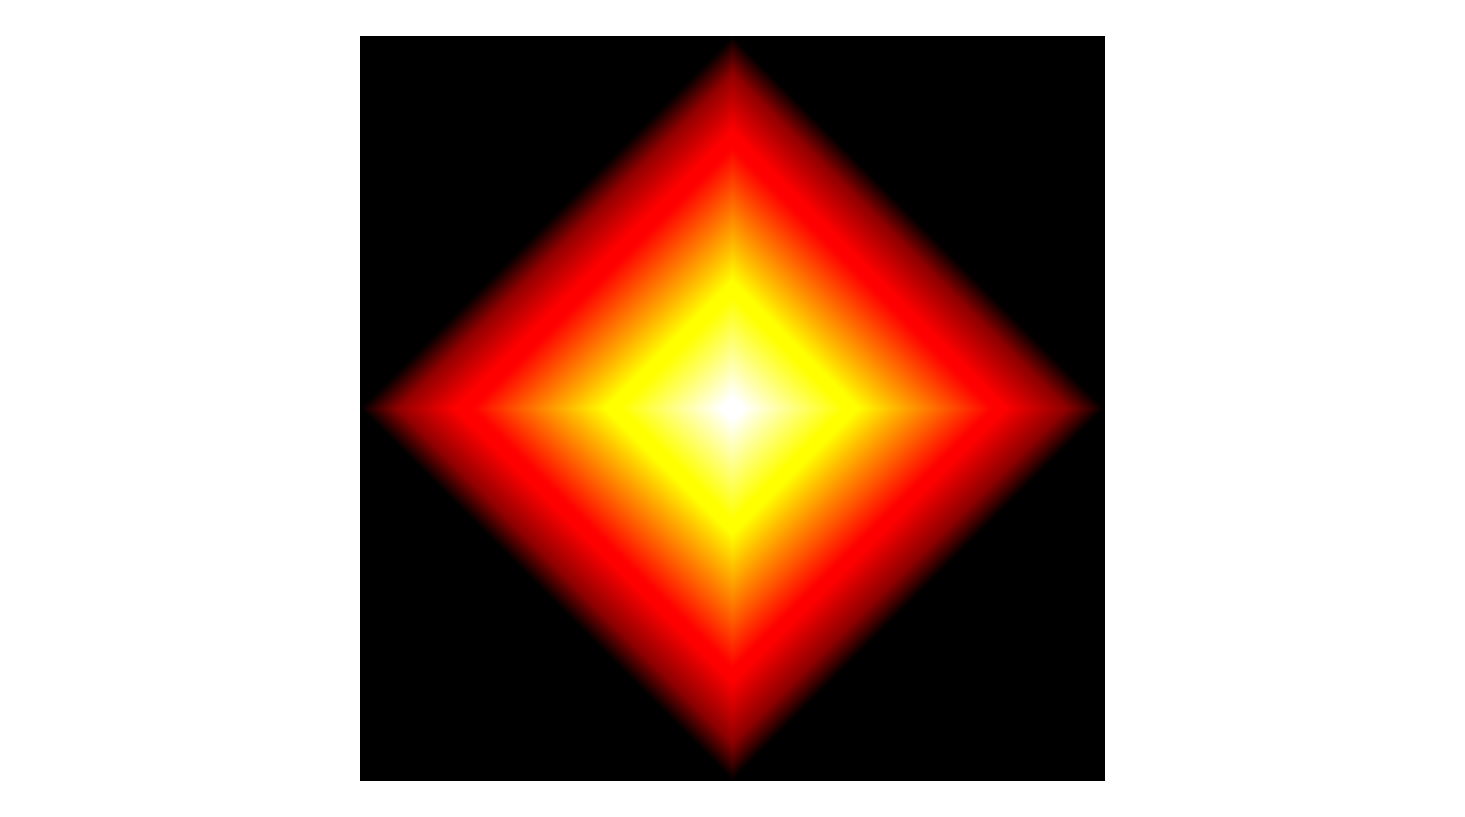
\includegraphics[width=\linewidth]
		{data/synthetic_meshes/square_tesselation_4tri_Dirac_delta_1_v13_f16_funcvals_0iter.png}
		\caption{R=1, convolutions 0}\label{fig:sq2.b}
	\end{subfigure}
	\begin{subfigure}[b]{0.32\linewidth}
		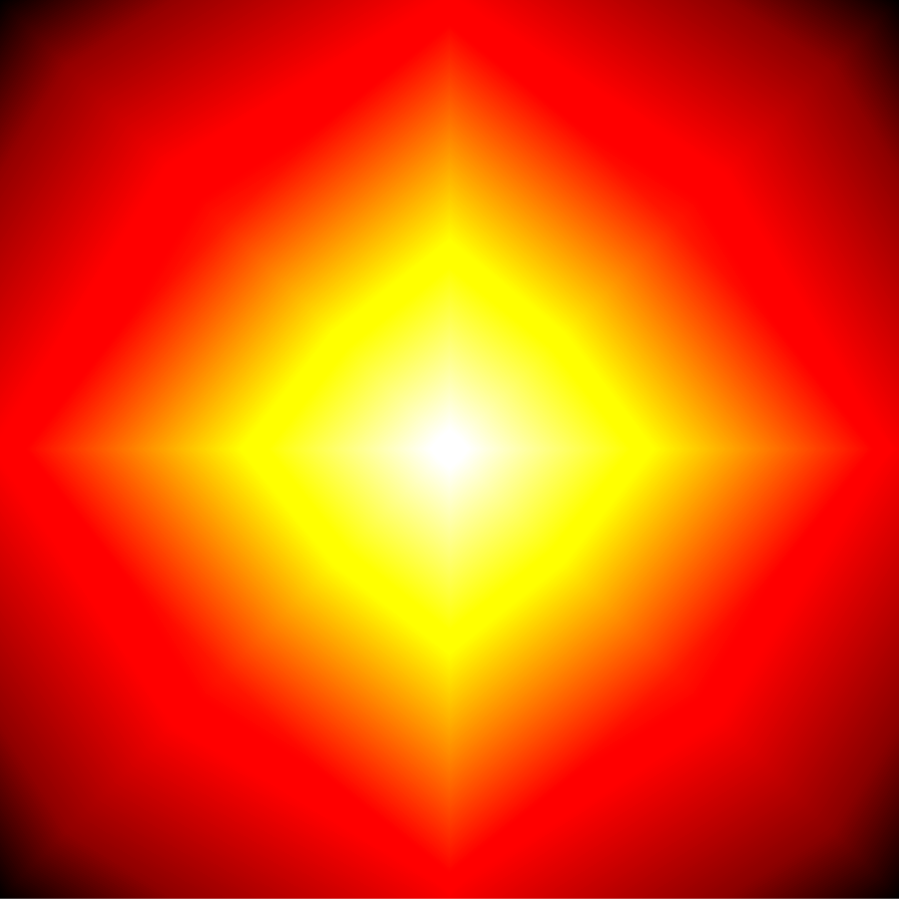
\includegraphics[width=\linewidth]
		{data/synthetic_meshes/square_tesselation_4tri_Dirac_delta_1_v13_f16_funcvals_1iter.png}
		\caption{R=1, convolutions 1}\label{fig:sq2.c}
	\end{subfigure}

	\bigskip
	\begin{subfigure}[b]{0.32\linewidth}
		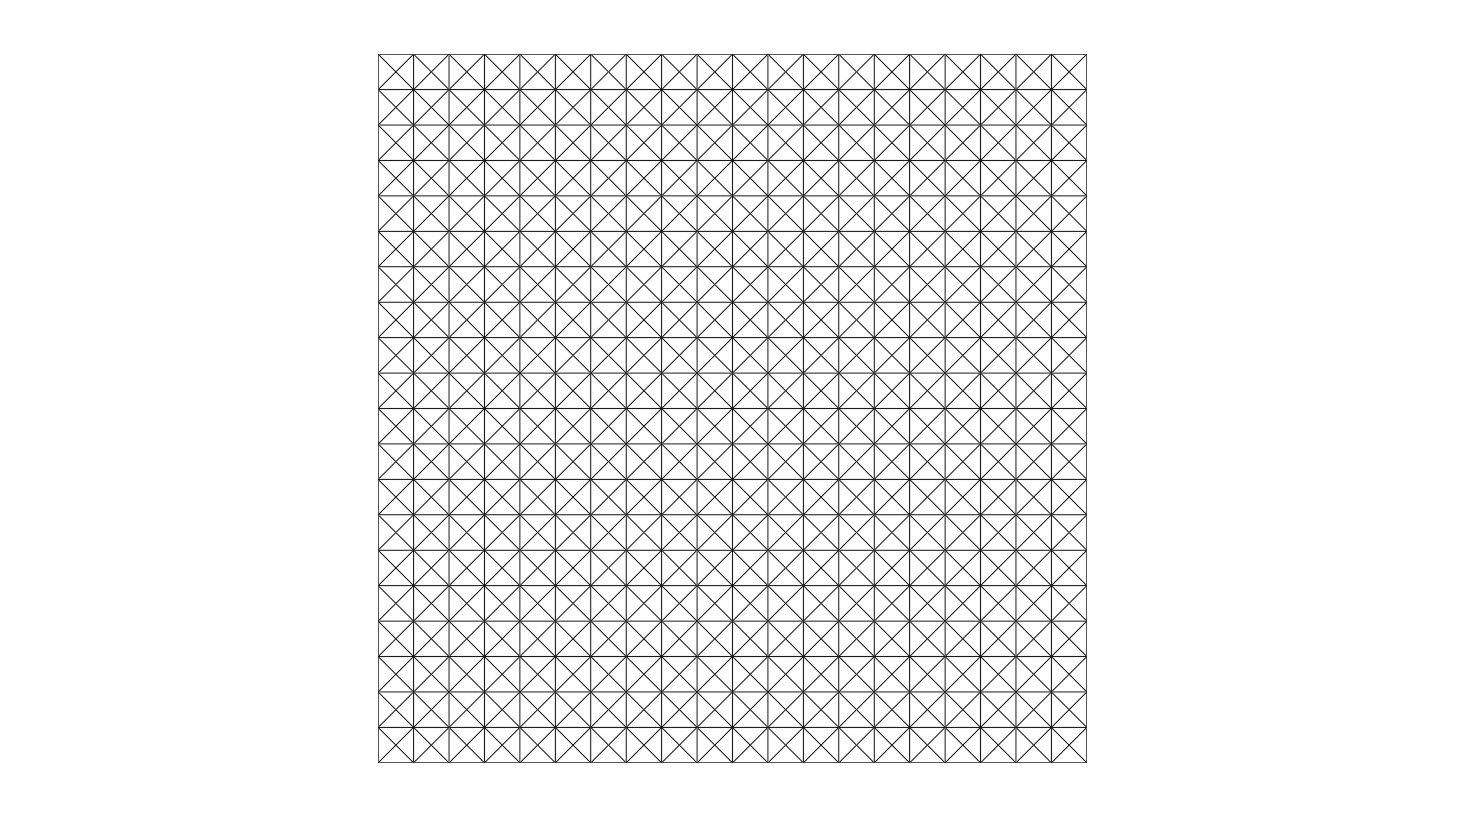
\includegraphics[width=\linewidth]
		{data/synthetic_meshes/square_tesselation_4tri_Dirac_delta_10_v841_f1600_wireframe.png}
		\caption{R=10, wireframe}\label{fig:sq2.d}
	\end{subfigure}
	\begin{subfigure}[b]{0.32\linewidth}
		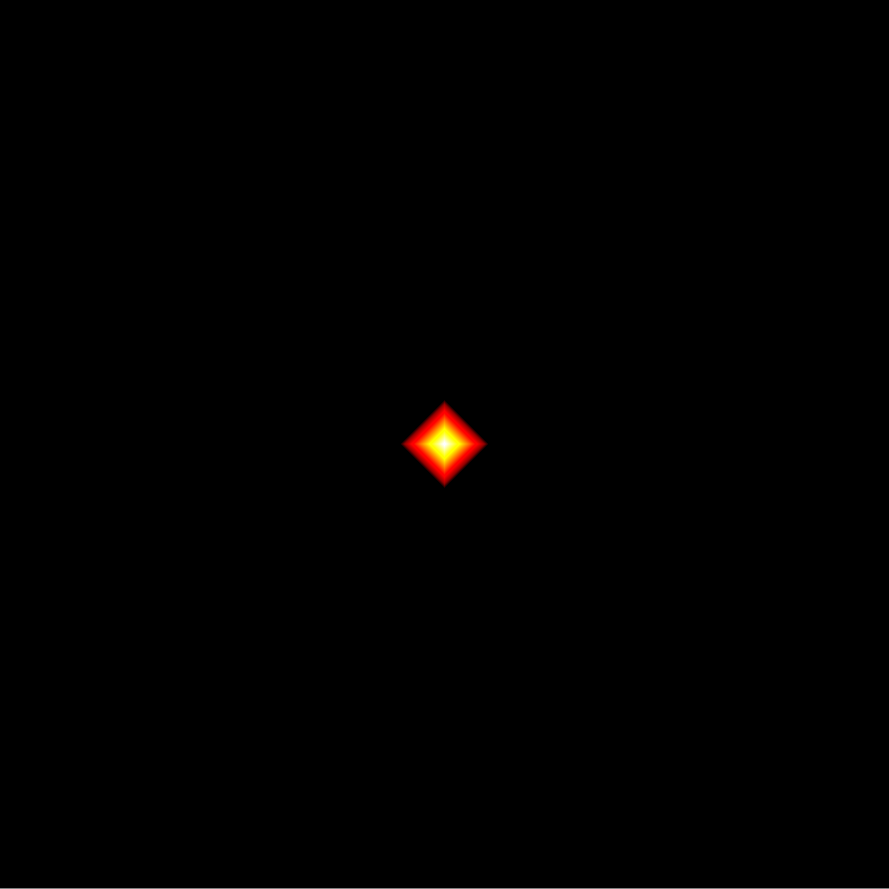
\includegraphics[width=\linewidth]
		{data/synthetic_meshes/square_tesselation_4tri_Dirac_delta_10_v841_f1600_funcvals_0iter.png}
		\caption{R=10, convolutions 0}\label{fig:sq2.e}
	\end{subfigure}
	\begin{subfigure}[b]{0.32\linewidth}
		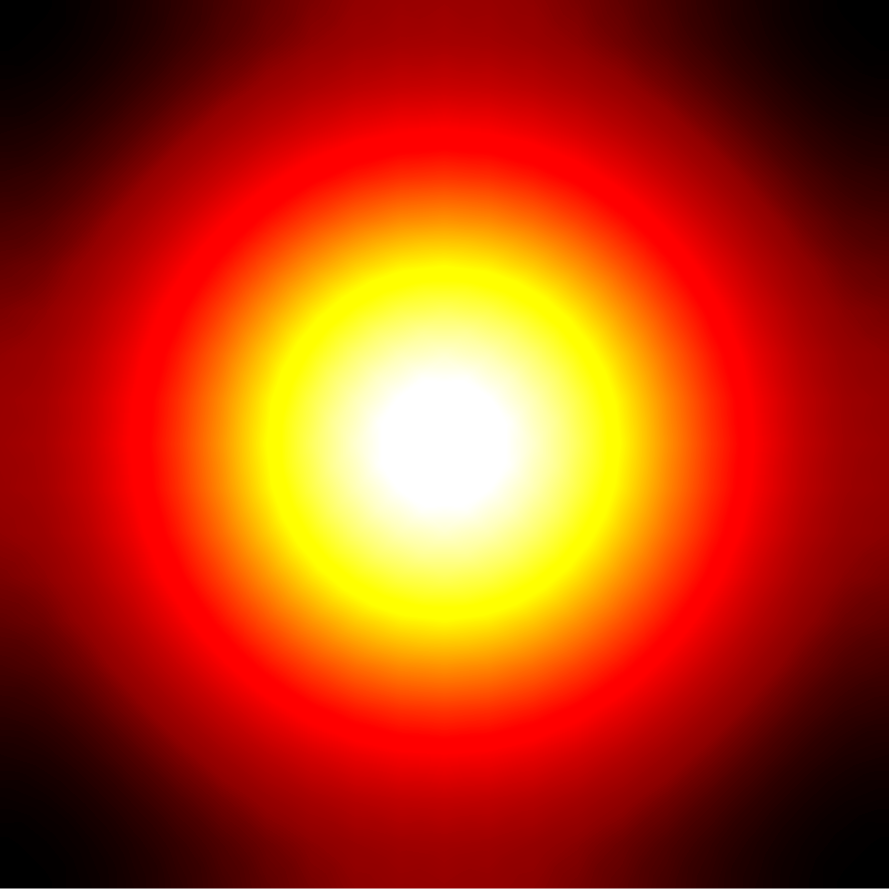
\includegraphics[width=\linewidth]
		{data/synthetic_meshes/square_tesselation_4tri_Dirac_delta_10_v841_f1600_funcvals_100iter.png}
		\caption{R=10, convolutions 100}\label{fig:sq2.f}
	\end{subfigure}
	\caption[Six views, comparing two differently sized of bisected square tessellations]{Comparison of two differently sized bisected square tessellations, generated with parameters R set to 1 and 10: (a) R=1 in wireframe (b) R=1 colored by function value before convolving the filter (c) R=1 colored by function value after convolving the filter once (d) R=10 in wireframe (e) R=10 colored by function value before convoving the filter (f) R=10 colored by function value after convolving the filter 100 times.}
	\label{fig:sq2}
\end{figure}
